%% Hello emacs, this is -*- latex -*-
\typeout{ ====================================================================}
\typeout{ This is file prefacio.tex, created at 13-Jun-2004 }
\typeout{ Maintained by Andre Rabello dos Anjos <Andre.dos.Anjos@cern.ch> }
\typeout{ ====================================================================}

\chapter{Introdução}
%%\addcontentsline{toc}{chapter}{\numberline{}Pref\'acio}

Sistemas eletrônicos de aquisição de dados são comumente empregados em muitos
campos da engenharia. Exemplos podem ser encontrados na captura de áudio,
vídeo, sinais de satélite, rádio, biológicos e cartográficos dentre outros. Os
sinais de fenômenos observados na natureza são registrados por sensores,
submetidos a uma conversão analógico-digital e processados por \eng{hardware}
especializado, programas rodando em computadores genéricos, sistemas dedicados
contendo DSP's, FPGA's ou misturas de todas essas tecnologias.

O número de sensores utilizados em cada nova situação varia de acordo com
problema abordado, podendo passar de alguns poucos (por exemplo, um microfone)
a uma quantidade gigantesca (o número de pixels em câmeras fotográficas
digitais). A informação pode se encontrar segmentada ou contida em um único
sinal que varia no tempo (e na freqüência). Em problemas extremamente
segmentados, é típica a utilização de pré-processamento distribuído,
habitualmente acoplado ao sensor. Unidades centralizadoras comunicam-se com a
eletrônica de aquisição de forma a obter os dados pré-processados e
combiná-los para gerar o resultado final esperado por aquele sistema.

Especificamente, em atividades relacionadas ao reconhecimento de padrões
captados por múltiplos sensores, a fase de pré-processamento é de extrema
importância. A informação dos sensores é recombinada em um espaço adaptado
onde a informação que se deseja discriminar torna-se mais evidente,
preferencialmente livre das correlações de ordem elevada que ocorrem
freqüentemente na natureza. Este processo de compactação ou extração de
características inteligente é normalmente desenvolvido tendo por base algum
conhecimento empírico sobre o sinal que será tratado. Exemplos clássicos
encontram-se no reconhecimento de imagens e voz, onde aplicam-se
transformações ao sinal original para aumentar a qualidade de discriminação
obtida nesses ambientes.

Em algumas instâncias, a deteção de padrões deve ser feita \eng{online}, em
janelas de tempo bastante limitadas. Como forma de aumentar a velocidade de
atuação destes detetores, é possível distribuir as tarefas de
pré-processamento e deteção em múltiplos processadores que trabalham
paralelamente para executar a tarefa de reconhecimento. Este cenário pode
ainda ser piorado se a informação estiver embebida em uma massa de dados muito
grande, que deva ser analisada para a deteção da informação procurada.

No caso de eventos raros serem o alvo do detetor, grande acurácia é exigida no
sistema de deteção, uma vez que a perda da informação de interesse pode
comprometer severamente a funcionalidade do sistema. Este é o caso, por
exemplo, de sistemas de apoio ao diagnóstico de doenças (como o câncer ou a
tuberculose) a partir de informações do paciente. O evento (doença) é raro,
mas deve ser detetado com acurácia.

\section{Motivação}

Experimentos em Física de Altas Energias procuram por confirmações
experimentais dos modelos propostos em estudos teóricos. Laboratórios deste
domínio da Física freqüentemente contam com um sistema de colisão, que provoca
o aparecimento da física de interesse associado a complexos sistemas de
deteção, que registram a evolução no tempo de cada evento
produzido. Naturalmente envolvidos no processo de deteção, encontram-se
sistemas eletrônicos que automatizam a busca, registro e análise dos
resultados obtidos.

Dada a natureza complexa e rara dos fenômenos estudados em muitos desses
experimentos, a física de interesse está normalmente submersa em uma
gigantesca massa de interações que representam ora ruído, provocados pelo mal
funcionamento dos sistemas de deteção e colisão, ora efeitos ordinários, já
bastante estudados no passado. Em específico, em experimentos que buscam a
confirmação de canais físicos em patamares energéticos elevados, de alguns
gigaelétron-volts para cima, a taxa de eventos que representa canais
desinteressantes contra a de eventos que possam interessar pode estar na
proporção de 10$^9$ para 1. Desta forma, as interações de interesse aparecem
escondidas no meio de bilhões de outras reações ordinárias, ou que representam
apenas ruído. Ademais, para que se consiga apreciar a Física de interesse,
milhões de eventos são gerados por base de tempo para que se colete
estatística suficiente para a comprovação do canal estudado. O volume de dados
associados a cada evento vem aumentando, junto com a ambição dos
experimentos. Novos sistemas de deteção exigem alguns \eng{megabytes} para
cada evento registrado, o que representa uma dificuldade extra na realização
desses experimentos.

Para resolver esse problema, introduzem-se sistemas eletrônicos de filtragem
que podem selecionar, de forma \eng{online}, os eventos de interesse dos
eventos que representam ruído ou física ordinária. Sua arquitetura é projetada
para resolver os desafios impingidos pelas duras condições de operação nestes
ambientes, seguindo os padrões de complexidade do experimento. Soluções atuais
empregam forte paralelização e técnicas modernas de processamento de sinais
para responder às demandas de colisões mais e mais energéticas.

Redes Neurais Artificiais vêm sendo empregadas nos sistemas de filtragem em
várias instâncias nessa área da Física. Dada a forte segmentação dos dados nos
detetores, sistemas neurais conseguem compactar e extrair as informações
vitais para a discriminação dos dados, mantendo não só a alta qualidade de
classificação como também excelentes níveis de velocidade de processamento.

\section{O experimento ATLAS e o bóson de Higgs}

A deteção do bóson de Higgs é um dos grandes expoentes da Física de Altas
Energias atual. Esta partícula, se existir, possui uma massa bastante elevada
(centenas de gigaelétron-volts) e se apresenta como um canal bastante raro e
de difícil reprodução laboratorial. A descoberta dessa partícula confirmará
mais uma vez o Modelo Padrão, já bastante testado, inicialmente proposto em
1954.

O CERN, na Suíça, é o local onde está sendo desenvolvido o experimento ATLAS,
que pretende investigar a rara física do bóson de Higgs. O experimento
utilizará colisões próton-próton, numa taxa de 40 milhões por segundo para
conseguir obter algumas dezenas destes bósons por dia de operação. As colisões
serão providas pelo Grande Colisionador de Hádrons (do inglês \eng{Large
Hadron Collider}, LHC), que será, quando estiver operacional, em 2007, o mais
potente no mundo, podendo colidir prótons com 14 TeV no centro de massa. Uma
vez que cada evento no ATLAS consumirá cerca de 1,5 \eng{megabytes} de espaço
em memória, um dos problemas do projeto e construção do experimento está na
articulação de um sistema de filtragem de eventos que seja capaz de fazer uma
seleção \eng{online} dos eventos que representem a Física de interesse.

O Sistema de Filtragem do ATLAS foi inicialmente projetado para
operar em três níveis conectados em cascata com complexidade, qualidade de
deteção e tempo de operação por evento, crescentes. O Segundo Nível de
Filtragem (LVL2), especificamente, será constituído de cerca de 1.000 unidades
de processamento ligadas em rede, processando cada candidato aprovado pelo
Primeiro Nível (LVL1). No LVL2 cada evento-candidato terá, em média,
aproximadamente 10 milissegundos para ser processado (latência).

O LVL2 coordena um conjunto de algoritmos descritos em \eng{software} que
executa a seleção de eventos. Dentre estes, algoritmos de deteção de elétrons
têm papel fundamental na eficiência da aquisição de dados, uma vez que a
ocorrência de elétrons pode representar a Física de interesse (em cerca de
60\% dos casos). Assim sendo, elétrons representam o sinal de interesse a ser
detetado. Estima-se que, a cada 25.000 candidatos a elétrons definidos pelo
LVL1, apenas 1 será verdadeiramente um elétron. Cabe ao LVL2 a redução deste
ruído de fundo significativo para a deteção de elétrons.

A informação para a deteção pode ser obtida do sistema de leitura do detetor
usando-se as primitivas do complexo \eng{software} de base do sistema de
filtragem, disponível em cada unidade de processamento dentro do LVL2. Os
dados para cada candidato a elétron são formados por células de deteção de um
calorímetro\footnote{Calorímetros são detetores especializados em amostrar a
energia das partículas que interagem com seu volume. Esses detetores serão
especificados e discutidos mais a frente no texto.}, segmentadas tanto na
direção de penetração da partícula, quanto no plano de interseção. Esse
sistema forma uma malha de elementos que contém amostras da energia de
interação da partícula sendo discriminada com o sistema de deteção ao longo
de sua trajetória. Em média, cada partícula-candidata ou ``objeto'' a ser
avaliado pelo LVL2, disporá de cerca de 1.300 células de deteção. A dimensão
flutuante de entrada, i.e., as diferenças no número total de células
analisadas para cada objeto, é devida a variações de granularidade do detetor
ao longo de seus eixos e outras facetas geométricas do experimento. Outras
causas que podem atingir a dimensão de entrada do sistema de discriminação
incluem defeitos no eletrônica do sistema de leitura do detetor ou transporte
dos dados até as unidades de processamento.

O processo de discriminação de cada objeto em si é dividido em duas etapas bem
definidas: a extração de características ou pré-processamento (fase 1) e a
deteção propriamente dita (fase 2), como mostra a
Figura~\ref{fig:intro-disc}. A extração de características visa a compactação
do sinal a ser detetado de forma que se realcem as proprieda
des necessárias à
deteção e reduza-se o espaço de entrada. A deteção propriamente dita, neste
caso, deverá ser simples e robusta de forma que o canal de interesse se
exprima claramente mesmo que embebido no rúido de fundo.

\begin{figure}
\begin{center}
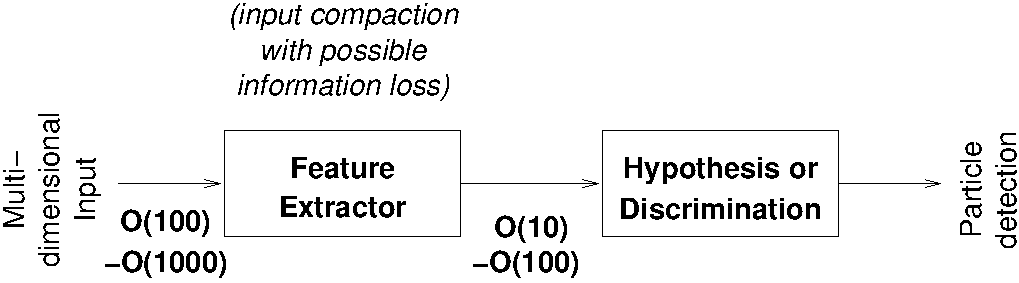
\includegraphics[scale=0.6]{basic-discriminator}
\end{center}
\caption{Um sistema genérico de deteção em um problema de Física de Altas
Energias.}
\label{fig:intro-disc}
\end{figure}

\section{Sobre as origens deste trabalho}

O experimento ATLAS foi iniciado em 1994 com a publicação de um relatório
técnico indicando o objetivo de sua existência (deteção do bóson de Higgs) e
sua complexa arquitetura em linhas gerais de operação. Desde então, as
arquiteturas de todos os sub-sistemas deste experimento foram modificadas
adaptando-se às novas tecnologias e aos desafios que surgiram com sua
manufatura, planejamento de transporte e construção. Algumas áreas sofreram
mudanças bastante radicais, como o sistema de filtragem, onde decidiu-se pela
utilização pioneira de computadores (PC's) e redes (ethernet) de tipo
doméstico atuando como unidades de processamento e interconexão desta parte do
experimento. Outras áreas foram afetadas de forma menos drástica, ainda que
bastante significativas, como no caso dos detetores, que tiveram suas
geometrias modificadas para aumentar a resolução na deteção das partículas de
interesse ou para remediar problemas relacionados à instalação.

Uma vez que os dados realísticos provenientes do ATLAS dependem de sua
instalação, áreas como o sistema de filtragem tiveram que ser desenvolvidos
baseados em simulações das reações que ocorrerão durante a operação do
experimento. De fato, este é um problema recorrente em experimentos em Físicas
de Altas Energias. Sistemas complexos de simulação existem e podem simular,
com detalhes impressionantes, reações subatômicas e a interação destas com
detetores formados de múltiplos materiais e módulos. As simulações da Física
de interesse e do ruído de fundo também foram amadurecendo com o passar dos
anos. Só atualmente é possível contar, por exemplo, com efeitos colaterais que
estarão presentes no experimento como ruído eletrônico ou o empilhamento de
informação (do inglês, \eng{pile-up}), causado pela sucessiva ocorrência de
colisões no interior do sistema de deteção. A geometria dos detetores na
simulação foi atualizada para casar com descrição do sistema (que já se
encontra instalado!), assim como os parâmetros de luminosidade que serão
esperados quando o LHC entrar em operação.

O trabalho discutido neste documento tem suas origens em 1995 com o Projeto
Final de gradução ``Sistema de classificação baseado em uma máquina com
sistema distribuído'', por este autor, apresentado em setembro de 1997
\cite{aa:projeto-final}. Os sistemas de deteção ainda estava sendo
desenvolvidos e poucas áreas tinham atingido um bom nível de maturidade. A
arquitetura do Sistema de Filtragem se encontrava, igualmente, em vias de
desenvolvimento.

Com base nas escolhas disponíveis na época, desenvolveu-se um sistema de
filtragem para o LVL2 baseado em um processamento distribuído, comandado por
um nó central de processamento, chamado Supervisor. As unidades de
processamento ou nós-escravos eram pré-carregadas com um sistema de deteção
neural. Estes nós analisavam os dados de cada evento atribuído pelo Supervisor
e distinguiam, \eng{online}, se o evento era interessante e deveria ser
aprovado por este nível de filtragem. No conjunto de dados disponível na
época, as características (após compactação) de cada objeto analisado já
haviam sido calculadas e, portanto, o sistema desenvolvido limitava-se ao papel
de \textit{deteção propriamente dita}, como colocado anteriormente.

No caso em questão, o Supervisor alocava, em \eng{round-robin}, os eventos a
cada uma das unidades de processamento que utilizavam o sistema neural para
avaliar as características de um objeto, determinando se o evento deveria ser
aprovado ou rejeitado. A resposta era enviada de volta ao Supervisor, que
simplesmente a registrava em um arquivo de saída. No final do processamento, a
saída registrada pelo Supervisor era comparada aos valores obtidos com um
programa \eng{offline} para que se determinasse se o sistema estava operando
corretamente.

Este modelo foi implementado em um máquina com 16 DSP's tipo T-9000@40~MHz, da
companhia INMOS. Cada nó de processamento continha, além das unidades lógicas
tradicionais, uma interface de rede especializada, com 4 canais independentes
de comunicação. O formato da interconexão entre os nós era configurável e foi
adaptado ao problema da distribuição dos dados entre o Supervisor e as
Unidades de Processamento. Para executar o \eng{boot} desta máquina, a
configuração de interconexão era carregada através de um sistema hospedeiro,
seguido de um \eng{micro-kernel} e, por final, um programa a ser
executado. Este programa podia ser codificado em C e compilado em um PC de
forma cruzada, para que fosse executado nos
\eng{transputers}.

Para essa implementação, o menor tempo de processamento para cada evento foi
390 microssegundos. O sistema de distribuição de eventos em
\eng{round-robin} garantia que 9 dos 15 nós de processamento estariam
executando uma tarefa dada em um instante tempo, o que era apenas sub-ótimo
tendo em vista as capacidades da máquina.

Com o passar dos anos, os diversos sistemas de deteção do experimento
começaram a se definir de forma mais concreta e os programas de simulação de
eventos físicos a ganhar detalhes e se aproximar, cada vez mais, de sua forma
atual. De posse de dados simulados de calorimetria relativos ao processamento
no LVL2, desenvolveu-se, de 1999 a 2001, também por este autor, o trabalho que
culminou na dissertação de mestrado entitulada ``Sistema neuronal rápido de
decisão baseado em calorimetria de altas energias'' \cite{aa:msc-thesis}.

Os dados disponíveis nesta época representavam cerca de 270 elétrons e 3600
jatos simulados através de interações simples com o detetor. O conjunto de
dados foi obtido a partir de uma simulação primitiva do sistema de deteção do
ATLAS e não continha diversos elementos que estarão presentes no sistema
de deteção final, tais como efeitos de ruído, empilhamento, variação de
granularidade e variação de energia.

A partir deste conjunto de dados, desenvolveu-se um sistema de discriminação
neural que pudesse operar dentro do Segundo Nível de Filtragem do ATLAS. Este
discriminador utilizava um pré-processamento em forma de anéis que se
aproveita do padrão de interação de elétrons com o detetor. Ao invés de
compactar o sinal da interação de elétrons com o detetor formando apenas 4
variáveis, como sugeria o sistema empregado no CERN naquela época, 58 variáveis
(anéis) eram produzidas. Um sistema de normalização simplificado, baseado na
energia total do objeto, foi empregado de forma que se removesse qualquer
tendência estatística provocada pela faixa estreita de energia presente nos
dados disponíveis.

O resultado da extração de anéis, normalizado, era utilizado como entrada para
um detetor neural com 58 neurônios de entrada, 5 neurônios na camada escondida
e apenas uma saída que indicava se o objeto na entrada era ou não um
elétron. A rede neural era treinada de forma supervisionada (usando-se o
método de retro-propagação clássica), utilizando-se metade do conjunto de
dados disponível. Neste caso, obteve-se 95\% de eficiência na deteção de jatos
contra 97\% para a deteção de elétrons. Este resultado foi comparado com uma
análise simplificada do sistema de deteção desenvolvido no CERN, que apontava
uma capacidade de discriminação de 95\% para elétrons para um falso-alarme de
11,6\% para jatos.

Uma análise baseada no impacto de cada um dos 58 anéis na saída da rede neural
(análise de relevância) revelou que era possível utilizar apenas 20 dos 58
anéis iniciais para uma deteção marginalmente inferior apenas àquela
utilizando todos os anéis, mas ainda muito superior à análise proposta no
CERN. Uma implementação simplificada do algoritmo foi executada, indicando a
possibilidade de ser utilizado no LVL2.

Atualmente, dispõe-se de um sistema muito mais elaborado para a simulação do
detetor ATLAS, e das colisões que acontecerão quando o acelerador for
finalmente ligado, em meados de 2007. Dentre os novos elementos presentes, se
encontram:

\begin{itemize}
\item Dimensão flutuante para os dados utilizados na deteção. No caso do
estudo para a dissertação de mestrado, limitou-se o escopo da análise a dados
com granularidade constante. Uma simulação muito mais realística do sistema de
deteção do ATLAS está presente na nova massa de dados, onde a granularidade da
região de interesse varia a cada camada e ao longo dos eixos do detetor,
trazendo um novo desafio a sistemas de deteção candidatos ao LVL2;

\item Introdução de ruído relativo ao sistema de deteção. Este efeito não
estava presente nos dados obtidos anteriormente, mas estará certamente
presente quando o experimento estiver operacional. A adição de ruído aos
sistemas de deteção diminui a acuidade das medidas, introduzindo uma
perturbação não desprezível aos algoritmos de deteção;

\item Um volume maior de dados está disponível para este trabalho, o que
possibilita uma análise muito mais detalhada e acurada do problema de deteção
elétron/jato. Enquanto que para os trabalhos anteriores dispunha-se de uma
massa muito limitada de dados, para este trabalho dispõe-se de aproximadamente
30.000 objetos (cerca de 22.500 elétrons e 7.500 jatos) para análise, o que
diminui a margem para possíveis erros estatísticos introduzidos por uma
análise sobre um conjunto de dados limitado;

\item A infrastrutura de suporte para o sistema de filtragem está
disponível. Todos os resultados, tanto de desempenho físico quanto velocidade
de processamento devem ser mencionados com relação a uma implementação
compatível e estável dentro desse ambiente. Dessa forma, é possível fazer o
sistema de deteção operar tal qual um algoritmo de deteção operaria no sistema
de filtragem e comparar seu desempenho tendo em vista todos os parâmetros
funcionais deste complexo ambiente;

\item O algoritmo empregado atualmente no CERN está também disponível em um
formato mais evoluído, em que seja possível uma comparação direta em termos de
eficiência e desempenho com um sistema alternativo. De posse dos resultados de
cada um dos algoritmos é possível conduzir uma análise mais detalhada das
diferenças entre os dois sistemas.
\end{itemize}

\section{As contribuições deste trabalho}

Este trabalho desenvolve e emprega métodos de análise multi-variável na
deteção de elétrons no Segundo Nível de Filtragem do experimento ATLAS. Isto é
feito tendo por base o modelo apresentado na Figura~\ref{fig:intro-disc}, onde
os métodos de extração de características (fase 1) são analisados tendo por
base sistemas de discriminação (fase 2) baseados em corte uni-dimensionais
sucessivos, detetores lineares, baseados na Análise de Componentes Principais
e Redes Neurais Artificiais. Os diversos sistemas são apresentados seguindo a
modelagem do processamento dentro do LVL2, como indica a figura.

Utiliza-se como base, o novo conjunto de simulações mais realísticas do
detetor e dos eventos que ocorrerão no ATLAS. Esta nova base de dados contém
um estrutura de eventos com granularidade variante e com muitos dos detalhes
operacionais do sistema de deteção final para o experimento. Estudos
detalhados de tendências estatísticas, para as diversas combinações de
compactadores e discriminadores, foram realizados levando-se em consideração a
energia das partículas ou sua localização no detetor (plano $\eta\times\phi$).

Inicialmente, levando-se em conta a massa de dados disponível, determinou-se a
eficiência de discriminação, que poderia ser obtida pelo sistema atualmente
empregado no CERN (fase 1 $+$ fase 2). Este sistema baseia-se na determinação
de 4 variáveis altamente discriminantes (algoritmo T2Calo, fase 1), seguido de
um processo de discriminação utilizando cortes unidimensionais (algoritmo
EGammaHypo, fase 2). Determina-se sua eficiência em $91,85\%$ para a deteção
elétrons contra um falso-alarme de $10,19\%$ em jatos.

Com base nestes ``valores canônicos de deteção'', observados com a análise
deste sistema de discriminação elétron/jato, desenvolve-se um detetor linear
para as 4 variáveis especialistas, substituindo-se o sistema de discriminação
\eng{ad-hoc} empregado no CERN. Este novo detetor tem um resultado
equivalente ao sistema anterior, indicando uma inseparabilidade linear,
inerente às variáveis no espaço compactado provido pelo algoritmo
T2Calo. Desenvolvemos então um detetor neural que atenda aos critérios da
filtragem de elétrons combinado a esse algoritmo de extração de
características. Esse novo sistema de discriminação apresenta uma eficiência
de classificação superior e também maior robustez na separação elétron/jato,
atingido $92,38\%$ na deteção de elétrons contra $9,05\%$ de falso-alarme.

Seguindo as tendências atuais de processamento neural aplicadas à Física de
Altas Energias, consideramos variáveis normalmente desprezadas para fins de
separação elétron/jato, mas produzidas durante o processo de compactação do
T2Calo, na criação de um novo sistema de discriminação mais eficiente. Este
novo sistema, utilizando 14 variáveis, obtém 94,79\% de eficiência na deteção
de elétrons contra uma taxa de falso-alarme de apenas 7,93\%, apresentando-se
ainda mais robusto que o sistema T2Calo (4 variáveis) $+$ detetor
neural. Nesse momento, conduzimos uma análise de relevância das variáveis que
revela que utilizando apenas 5 das 14 variáveis iniciais é possível
desenvolver um detetor tão eficiente quanto aquele usando as 14 variáveis.
Observando-se as correlações existentes entre as 14 variáveis, conduzimos uma
Análise de Componentes Principais no objetivo de remover correlações no espaço
de entrada do detetor neural, aumentando dessa forma, o nível de compactação
que poderia ser obtido.

Conduz-se então uma análise baseada no pré-processamento em anéis. Para esta
análise, um novo sistema de mapeamento das informações do detetor em anéis foi
elaborado, levando-se em consideração vários aspectos que ainda não haviam
sido abordados: a problemática dos dados faltantes, a introdução de ruído
proveniente da eletrônica, a variação de granularidade dentro da camada e
camada a camada. Com base neste pré-processamento, 100 variáveis
correspondentes aos anéis são extraídas de cada objeto a ser analisado. Um
detetor neural é elaborado para a fase de deteção propriamente dita,
levando-se em consideração uma otimização do espaço de parâmetros para seu
treinamento. Este novo sistema obtém uma eficiência de classificação de
elétrons de $96,55$\% contra apenas $3,12$\% de falso-alarme. Uma análise de
relevância baseada das variáveis de entrada (anéis) ao detetor neural é
conduzida tendo em vista seu poder de discriminação. Finalmente, um detetor
utilizando apenas 14 dos 100 anéis iniciais é desenvolvido, baseando-se na
relevância discriminativa dos anéis de deposição energética. Este sistema
atinge uma eficiência de $97,59$\% na deteção de elétrons contra um falso
alarme de $3,22$\%.

Atualmente, algoritmos candidatos ao Sistema de Filtragem devem suprir não
somente condições de eficiência, mas também de tempo de execução, se
integrando perfeitamente à pilha de \eng{software} do ATLAS. Uma vez tendo
desenvolvido o sistema de deteção, o integramos a esta infraestrutura de
processamento completamente, de forma a verificar sua portabilidade, tempo de
processamento e acuidade, enquanto embebido no inóspito ambiente de deteção do
ATLAS. Testes de velocidade e exatidão são conduzidos em várias plataformas,
donde se conclui que o sistema baseado em análise multi-variável seja viável
para implementação no segundo nível de filtragem do experimento. Enquanto o
sistema atual empregado no CERN consome cerca de 3,64 milissegundos para ser
executado, o sistema baseado na extração em anéis e deteção neural, mais que 3
vezes mais eficiente na rejeição de falsos-positivos, é executado em 3,8
milissegundos dentro da mesma infraestrutura de base, apenas cerca de 150
microssegundos de diferença em média. Finalmente, uma implementação baseada em
DSP's é derivada, indicando uma nova plataforma de desenvolvimento e a
portabilidade desejada ao sistema.

Este trabalho foi desenvolvido com o objetivo de avaliar novas técnicas de
deteção para o experimento ATLAS, no contexto da colaboração internacional
entre o CERN e a UFRJ. As contribuições deste trabalho também incluem o
desenvolvimento e a construção de boa parte do Segundo Nível de Filtragem e sua
infrastrutura \eng{online}, que serão narradas como um contínuo no decorrer do
texto. Dentre as mais significativas, podemos destacar:

\begin{enumerate}
\item Desenvolvimento e aplicação da Unidade Central de Processamento no
LVL2, a L2PU;
\item Desenvolvimento e aplicação da biblioteca global de formatação de dados
do ATLAS (\eng{eformat});
\item Desenvolvimento e aplicação do \eng{Pseudo} Sistema de Leitura (PROS);
\item Desenvolvimento e aplicação de uma biblioteca para rápido acesso e
processamento de dados de calorimetria;
\item Desenvolvimento e aplicação da camada de \eng{software} que combina a
L2PU e a suíte de processamento \eng{offline} Athena;
\item Medidas de desempenho do sistema de filtragem para diferentes cenários,
com ou sem a utilização de algoritmos de discriminação.
\end{enumerate}

\section{Organização do Texto}

O Capítulo~\ref{chap:introducao} traz uma visão geral da Física de Partículas
atual. Este capítulo inicia-se sumarizando fatos histórios que culminaram na
formulação do Modelo Padrão para a descrição das interações sub-atômicas. Em
seguida, é feita uma revisão das técnicas de aceleração e deteção de
partículas mais comuns em experimentos nessa área. Na
Seção~\ref{sec:calorimetria} descrevem-se detetores conhecidos como
\textit{calorímetros} em maiores detalhes. Aqui, discutem-se as partículas de
interesse para o trabalho e a forma como interagem com este tipo de detetor. O
capítulo termina introduzindo noções gerais sobre os sistemas de filtragem que
equipam os experimentos modernos.

O Capítulo~\ref{chap:atlas} narra especificidades do experimento ATLAS, que
investigará a Física do bóson de Higgs. O capítulo é encabeçado por um breve
histório do CERN, adentrando por detalhes operacionais do experimento e do
colisionador LHC, que gerará as interações próton-próton necessárias. A
Seção~\ref{sec:atlas-calo} traz um resumo das características operacionais dos
Calorímetros do ATLAS e um conjunto de referências para maiores detalhes.

O Sistema de Filtragem do ATLAS é introduzido no
Capítulo~\ref{chap:trigger}. Este capítulo descreve todos os sub-sistemas que
compõem o Sistema de Filtragem do experimento, desde o Primeiro Nível de
Filtragem até chegar à gravação de um evento selecionado em mídia
permanente. É neste ambiente que são executados os algoritmos de filtragem
abordados neste trabalho. O Segundo Nível de Filtragem e algumas das
contribuições deste trabalho são detalhados a partir da
Seção~\ref{sec:lvl2arch}. Resultados obtidos durante simulações do
comportamento desta parte do sistema são apresentados na
Seção~\ref{sec:lvl2work}. O final deste capítulo é dedicado ao ambiente de
processamento de dados Athena e sua interação com o Sistema de Filtragem do
ATLAS. Neste capítulo descreve-se em detalhes os componentes de infraestrutura
produzidos no contexto da colaboração entre o CERN e a UFRJ.

O Capítulo~\ref{chap:baseline} apresenta os aspectos da filtragem elétron/jato
conduzida no experimento ATLAS, partindo do LVL1 até que os eventos estejam
disponíveis no LVL2. O algoritmo de deteção de elétrons nesses dois níveis de
filtragem são avaliados em detalhes. O capítulo termina com uma análise
completa do algoritmo do LVL2, tendo por base os dados utilizados durante este
trabalho de tese.

O Capítulo~\ref{chap:neural} começa trazendo uma revisão das técnicas de
análise multi-variáveis que são atualmente empregadas em experimentos em Física
de Altas Energias, especialmente focado no emprego de redes neurais em
calorimetria. O texto continua desenvolvendo os diversos sistemas de
discriminação propostos. Na primeira parte, com sistemas baseados na
re-utilização do algoritmo de extração de características T2Calo e, numa
segunda, utilizando um processamento baseado em anéis de deposição energética
remodelado e melhorado.

O Capítulo~\ref{chap:implement} adentra pelo emprego do sistema desenvolvido
no capítulo anterior, dentro do Sistema de Filtragem do ATLAS. Demonstra-se
que é possível construir e executar sistemas de deteção neural dentro desse
complexo ambiente. Testes de acuidade e velocidade são conduzidos e analisados
em diversas plataformas. Este capítulo termina com a descrição de uma
implementação do sistema de anelamento e deteção neural em DSP's.

O Capítulo~\ref{chap:conclusions} traz uma conclusão dos estudos realizados e
apresenta extensões de estudo para este trabalho.

Para a melhor compreensão dos termos utilizados na descrição da geometria dos
objetos estudados neste trabalho, o Apêndice~\ref{ap:coord} introduz o sistema
de coordenadas do ATLAS. O Apêndice~\ref{ap:framework} sumariza os detalhes de
implementação do pacote de \eng{software} \texttt{Neuralringer}, utilizado
para as medidas de eficiência, relevância e que foi transplantado para
operação dentro do Sistema de Filtragem do experimento. Finalmente, o
Apêndice~\ref{ap:published} traz um resumo da produção científica durante o
período.

\typeout{ *************** End of file prefacio.tex *************** }
